%\title{LaTeX Portrait Poster Template}
%%%%%%%%%%%%%%%%%%%%%%%%%%%%%%%%%%%%%%%%%
% a0poster Portrait Poster
% LaTeX Template
% Version 1.0 (22/06/13)
%
% The a0poster class was created by:
% Gerlinde Kettl and Matthias Weiser (tex@kettl.de)
% 
% Adapter by Jens Buysse for Hogeschool Gent
% This template has been downloaded from:
% http://www.LaTeXTemplates.com
%
% License:
% CC BY-NC-SA 3.0 (http://creativecommons.org/licenses/by-nc-sa/3.0/)
%
%%%%%%%%%%%%%%%%%%%%%%%%%%%%%%%%%%%%%%%%%

%----------------------------------------------------------------------------------------
%	PACKAGES AND OTHER DOCUMENT CONFIGURATIONS
%----------------------------------------------------------------------------------------

\documentclass[a0,portrait]{a0poster}

\usepackage{multicol} % This is so we can have multiple columns of text side-by-side
\columnsep=100pt % This is the amount of white space between the columns in the poster
\columnseprule=3pt % This is the thickness of the black line between the columns in the poster

\usepackage[svgnames]{xcolor} % Specify colors by their 'svgnames', for a full list of all colors available see here: http://www.latextemplates.com/svgnames-colors

\usepackage{times} % Use the times font
%\usepackage{palatino} % Uncomment to use the Palatino font

\usepackage{graphicx} % Required for including images
\graphicspath{{figures/}} % Location of the graphics files
\usepackage{booktabs} % Top and bottom rules for table
\usepackage[font=small,labelfont=bf]{caption} % Required for specifying captions to tables and figures
\usepackage{amsfonts, amsmath, amsthm, amssymb} % For math fonts, symbols and environments
\usepackage{wrapfig} % Allows wrapping text around tables and figures
\usepackage[export]{adjustbox}

\begin{document}

%----------------------------------------------------------------------------------------
%	POSTER HEADER 
%----------------------------------------------------------------------------------------

% The header is divided into two boxes:
% The first is 75% wide and houses the title, subtitle, names, university/organization and contact information
% The second is 25% wide and houses a logo for your university/organization or a photo of you
% The widths of these boxes can be easily edited to accommodate your content as you see fit

\begin{minipage}[t]{0.75\linewidth}
\VeryHuge \color{HoGentAccent1} \textbf{Microservice Integration Patterns op SAP order-to-cash proces} \color{Black}\\ % Title
\huge \textbf{Van Damme Lyva, Nicolas Pauwelyn, Karine Samyn}\\[0.5cm] % Author(s)
\huge Hogeschool Gent, Valentin Vaerwyckweg 1, 9000 Gent\\[0.4cm] % University/organization
\Large \texttt{lyva.vandamme.y7102@student.hogent.be} \\
\end{minipage}
%
\begin{minipage}[t]{0.25\linewidth}

\includegraphics[width=13cm,right]{figures/HOGENT_Logo_Pos_rgb.png} 

\end{minipage}

\vspace{1cm} % A bit of extra whitespace between the header and poster content

%----------------------------------------------------------------------------------------

\begin{multicols}{2} % This is how many columns your poster will be broken into, a portrait poster is generally split into 2 columns

%----------------------------------------------------------------------------------------
%	ABSTRACT
%----------------------------------------------------------------------------------------

\color{HoGentAccent1} % Navy color for the abstract

\begin{abstract}
Dit onderwerp, hoe microservices invloed hebben op het SAP order-to-cash proces, werd voorgesteld door delaware. Dit werd gekozen omdat deze nieuwe technology een interessante invloed kan hebben op de order-to-cash proces. Dit is een manier om een proces robuuster te maken. In de meeste software wordt gebruik gemaakt van één grote databank of meerdere databanken
die in staan zijn om meerde services te voorzien van data. Bij microservices wordt voor elke service een aparte databank opgesteld. Dit is maar een klein deeltje van een microservice. De microservice moet voldoen aan business requirements. SAP zelf heeft ook al veel ondernomen omtrend microservices. Eén van hun oplossingen is Kyma. Maar de belangrijkste vraag is namelijk: Hoe microservice integration patterns een SAP order-to-cash beïnvloedt. \end{abstract}
%----------------------------------------------------------------------------------------
%	INTRODUCTION
%----------------------------------------------------------------------------------------
\color{Black} % DarkSlateGray color for the rest of the content
\color{HoGentAccent1} 
\section{Waar en wanneer?}
Om 14u30 in lokaal B3.026

\color{HoGentAccent1} 
\section*{Introductie}
\color{black}
\color{black}
\subsection{Waarom microservices?}
De architectuur maken aan de hand van microservice patroon of aan de hand van monolithic? Een vraag die wel vaker gesteld wordt. Afstappen van het iets dat we kennen? Een sprong in het donkere, het onbekende. Een microservice architecture brengt voordelen en nadelen met zich mee, net zoals monolithic. Maar waarom kiezen we de microservice techniek boven die van monolithic? En welke passen heeft SAP al genomen om hun klanten de mogelijkheid van microservices aan te bieden?

\subsection{Waarom order-to-cash proces?}
Het order-to-cash proces is een veel gebruikt proces binnen bedrijven. Dit proces heeft veel invloed op het succes van een bedrijf. Er kan aangetoond worden hoe het proces beïnvloedt wordt door microservices. Welke obstakels er waren bij het uitdenken van de architectuur. Waar waren er problemen, waar moest er meer nagedacht worden over een oplossing? Een order-to-cash proces wordt over verschillende afdelingen gebruikt. Dit is een reden om dit proces uit te kiezen. Het proces bevat onderdelen die verschillende doelen hebben.
%----------------------------------------------------------------------------------------
%	GEOLOGY
%----------------------------------------------------------------------------------------

\color{Black} % DarkSlateGray color for the rest of the content
\color{HoGentAccent1} 
\section*{Experimenten}
\color{black}
Deze bachelorproef was een theoretisch onderzoek naar de invloed van microservices op een order-to-cash proces. Er werd onderzoek uitgevoerd naar op welke manier er moest worden overgeschakeld worden. Welke communicatie methode er kan gebruikt worden tussen de microservices. Het volledige proces werd opgesplitst. Er werd nagegaan welke requirements elk onderdeel van het proces had. 
Er werd een uitgebreide literatuurstudie gedaan over microservices. Dit is een breed onderwerp. Er is diep ingegaan op bepaalde eigenschappen van microservices. De term zelf is heel breed.



\color{HoGentAccent1} 
\section*{Sectie met figuur}
\color{black}


\begin{center}\vspace{1cm}
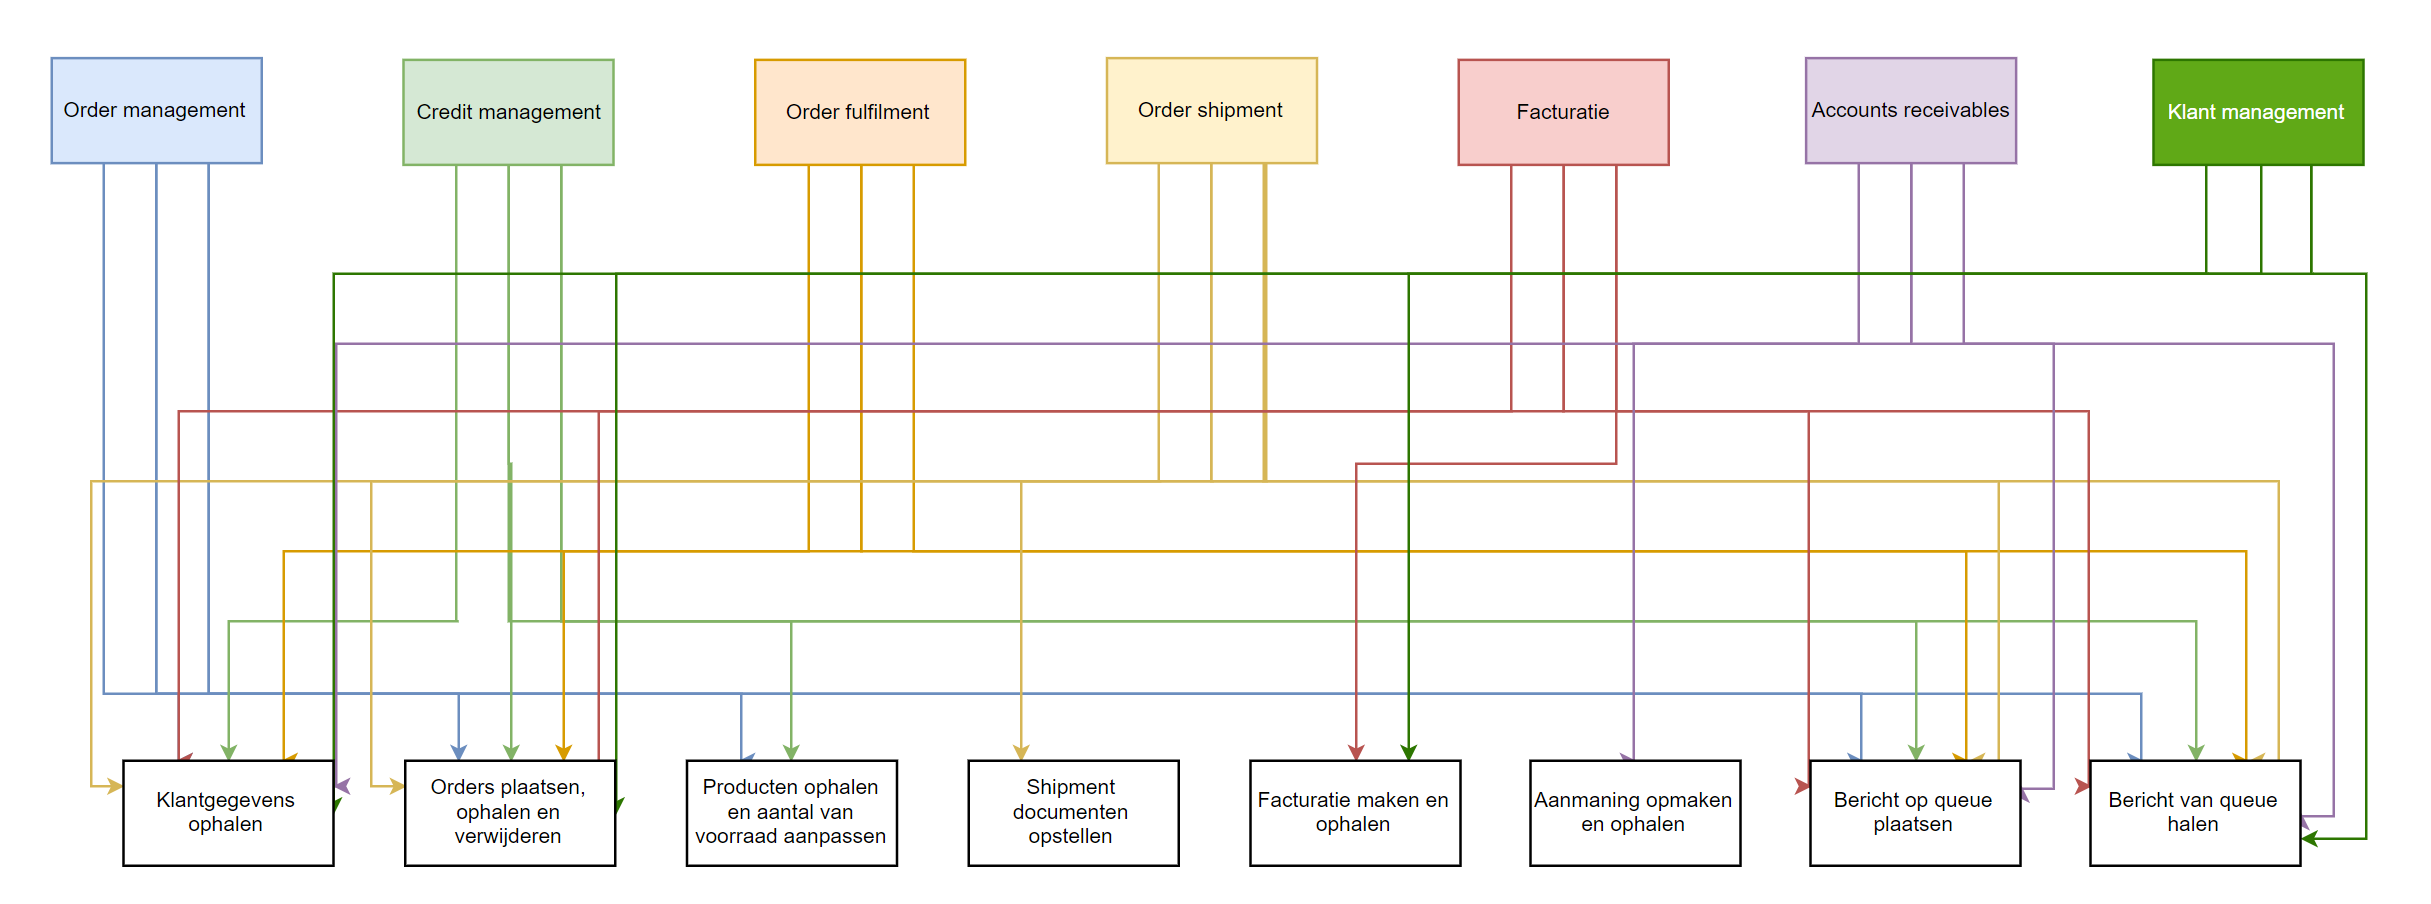
\includegraphics[width=1.0\linewidth]{schema_microservices}
\captionof{figure}{\color{HoGentAccent5} Het order-to-cash proces waarvan elk onderdeel zijn nodige microservices aanspreekt.}
\end{center}\vspace{1cm}

%------------------------------------------------



\color{HoGentAccent1} 
\section*{Conclusies}
\color{black}
Microservice is een architectuur en ideologie waarin logica en de requirements, die te
vinden zijn bij een monolithic, terugkomen. Dit heeft invloed op de overschakeling naar
microservices. Deze manier van implementatie moet aangepast worden bij het gebruik
van microservices. Dat kan een obstakel zijn. Er wordt een andere manier van denken
en organiseren gevraagd binnen een de IT-afdeling. De teams worden hervormd. Een
team bevat niet meer de kennis van de volledige architectuur., enkel over de microservice
waaraan zij werken.

De performance zal stabieler zijn bij pieken van orders. Omdat de microservices
onafhankelijk zijn van elkaar. De onderdelen van het OTC proces kunnen onafhankelijker
functioneren. Valt er een onderdeel uit of tijdelijk niet beschikbaar dan heeft dat geen
grote gevolgen voor het proces in het algemeen. Het onderdeel ervoor kan nog altijd data
op de queue plaatsen. Maar de onderdelen na het onbeschikbare deel, zal wel wat hinder
ondervinden. Maar niet zodat het gehele proces plat zal liggen.
%----------------------------------------------------------------------------------------
%	FORTHCOMING RESEARCH
%----------------------------------------------------------------------------------------
\color{HoGentAccent1} 
\section*{Toekomstig onderzoek}
\color{black}
In de toekomst kan er een proof of concept gemaakt worden. De verschillende communicatie methodes kunnen verder onderzocht worden. De manier om authenticatie en authorisatie toe te passen, kunnen nog dieper worden onderzocht. Deze studie probeerde zo veel mogelijk eigenschappen van microservices aan te halen. Dit zogrt ervoor dat er niet op elk deel diep kan worden ingegaan. In de toekomst kan elk deel van microservices dieper worden onderzocht en uitgetest.


%----------------------------------------------------------------------------------------

\end{multicols}
\end{document}